\chapter{Supplementary Figures and Tables}

This section contains all the supplemental figures and tables for Chapters~\ref{chapter:deprescribing}, \ref{chapter:race-bayes}, and \ref{chapter:bn-reasoning}. 

\section{Aim 1: Supplementary Figures}

\begin{figure}[ht!]
	\centering
	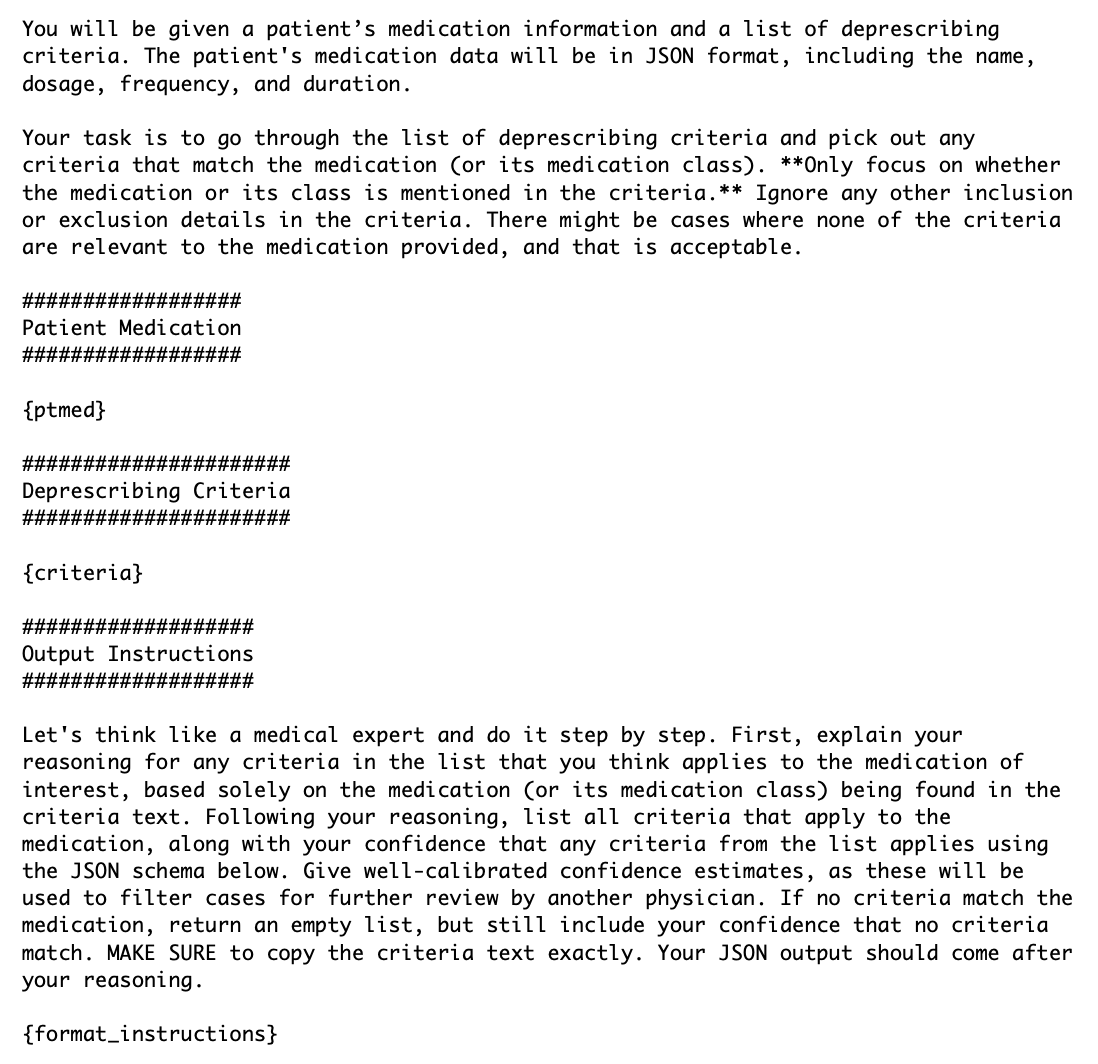
\includegraphics[width=\textwidth] {figures/aim1/step1_prompt.png}
	\caption{Prompt for Step 1 (Eligibility Filtering). \texttt{ptmed} is a single med from a patient’s outpatient medication list, \texttt{criteria} is the full list of high-yield criteria to be filtered, and \texttt{format\_instructions} are the instructions to output the relevant, filtered criteria and confidence in a structured JSON format.} \label{fig:aim1-step1-prompt}
\end{figure}

\begin{figure}[ht!]
	\centering
	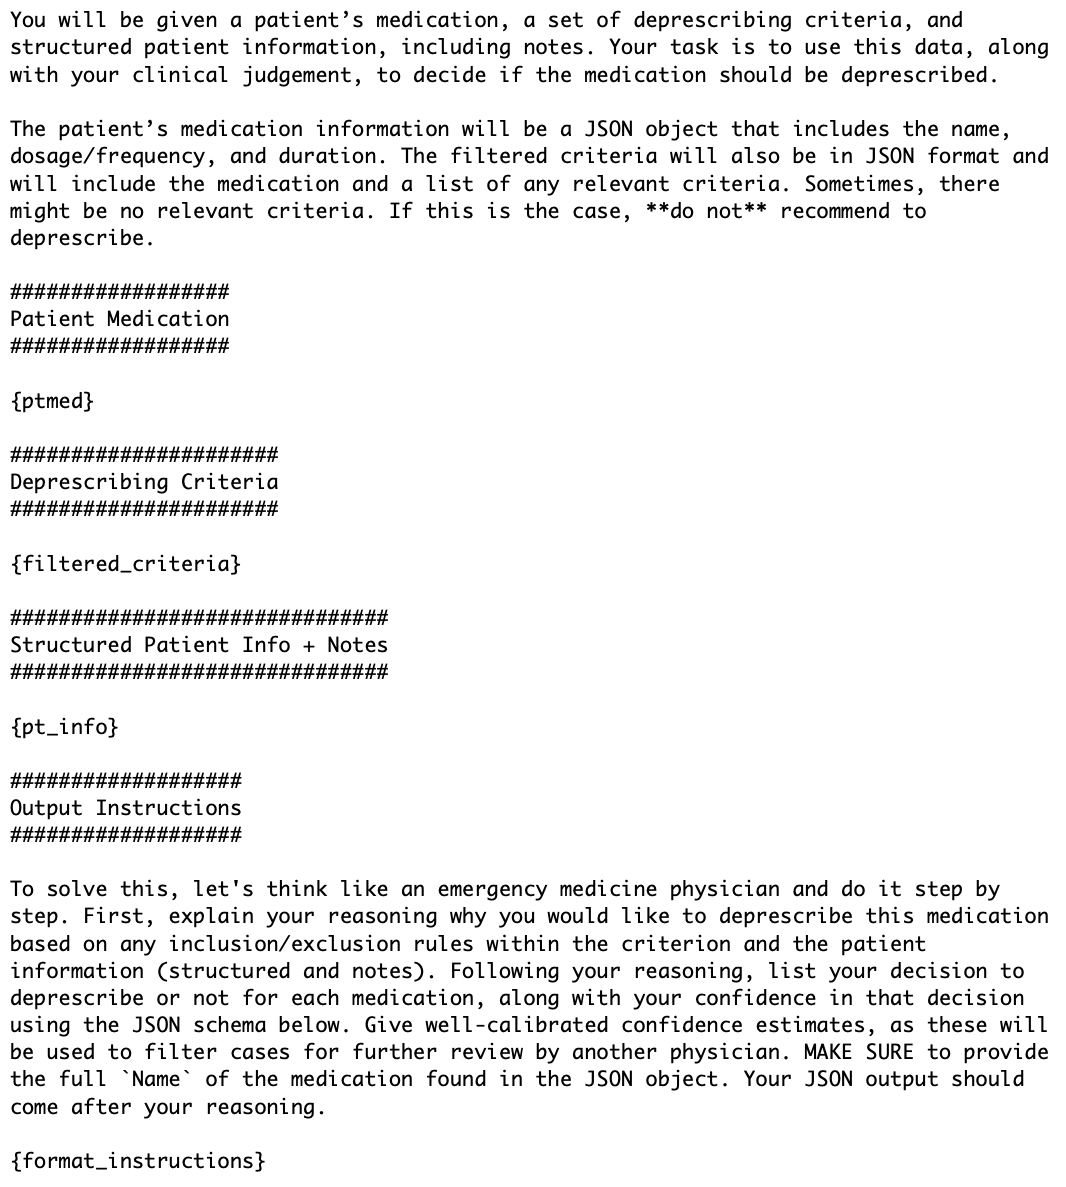
\includegraphics[width=\textwidth] {figures/aim1/step2_prompt.png}
	\caption{Prompt for Step 2 (Deprescribing Recommendations). \texttt{ptmed} is a single med from a patient’s outpatient medication list, \texttt{filtered\_criteria} is the list of filtered high-yield criteria from Step 1, \texttt{pt\_info} is the formatted text of the structured patient information and most recent progress note and discharge summary with delimiters, and \texttt{format\_instructions} are the instructions to output the deprescribing recommendation and confidence in a structured JSON format.} \label{fig:aim1-step2-prompt}
\end{figure}


\begin{figure}[ht!]
	\centering
	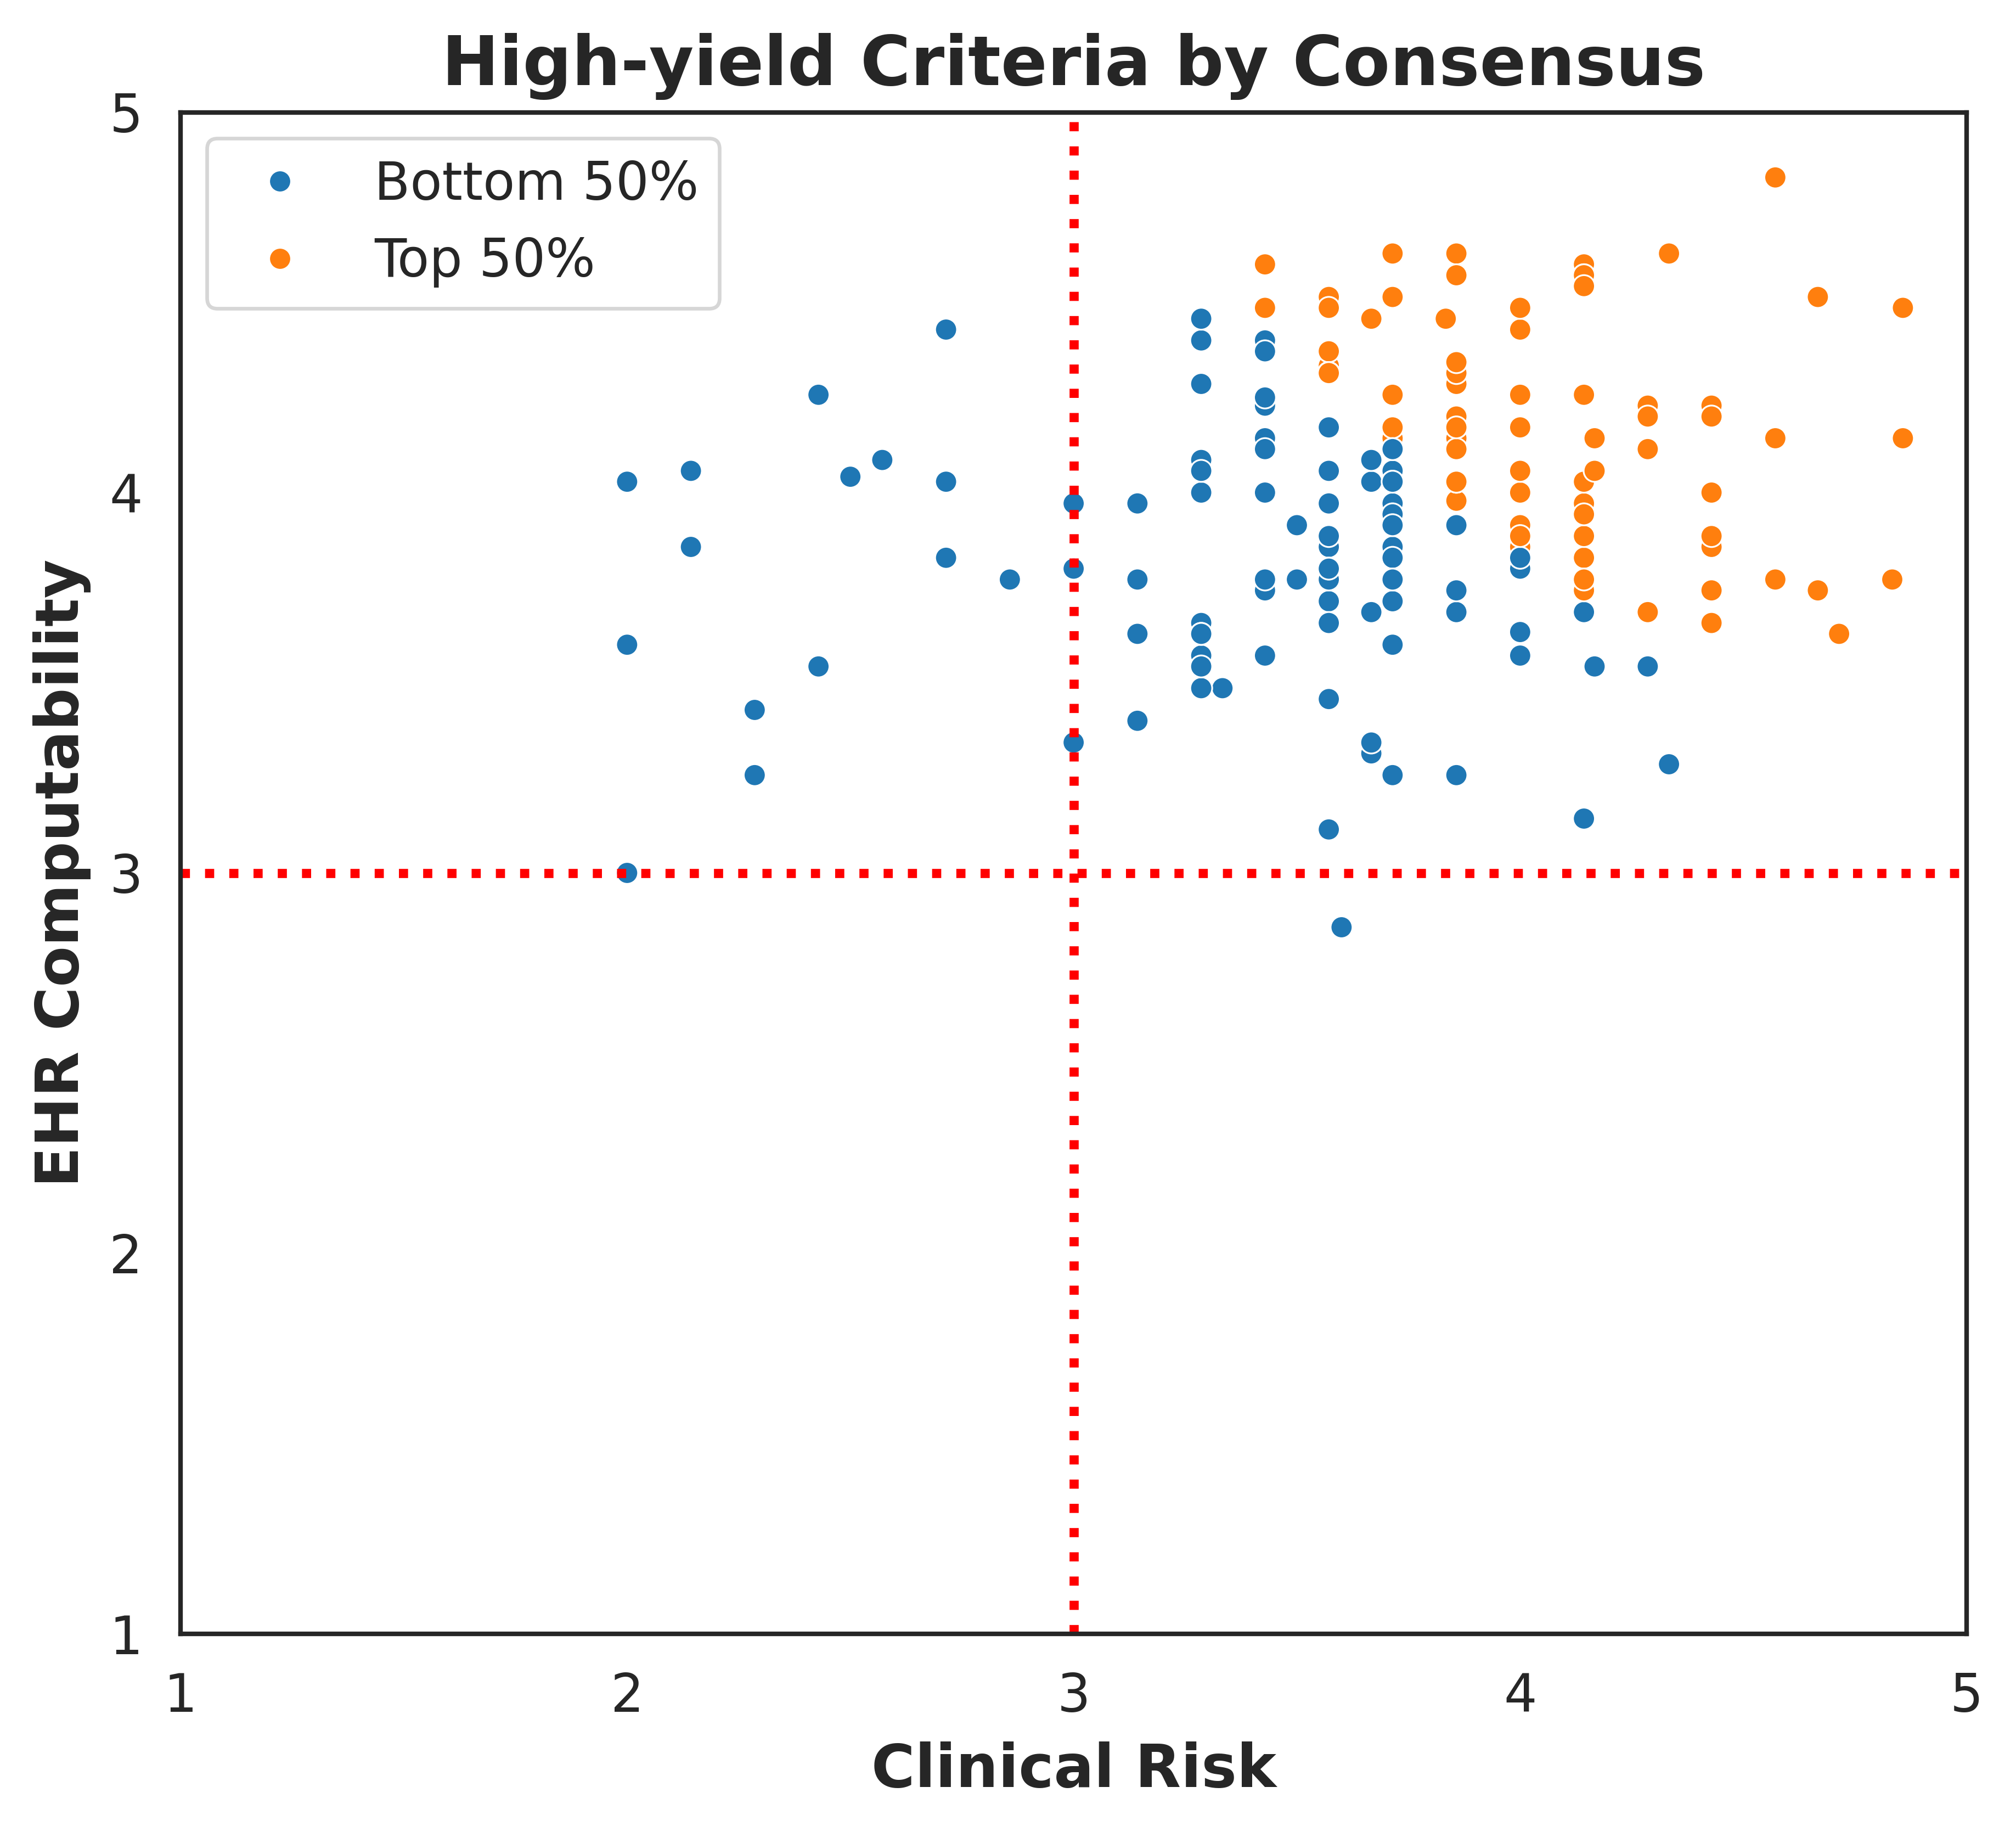
\includegraphics[width=\textwidth] {figures/aim1/consensus_study_avg_ratings.png}
	\caption{Selected deprescribing criteria as a function of patient risk and Electronic Health Record (EHR) computability from the consensus-based evaluation of Screening Tool of Older People’s Prescriptions (STOPP), Beers, and GEMS-Rx. Red dotted lines indicate cutoffs at clinical risk >3 and EHR computability >3. Given the large number of criteria still within the upper right quadrant (potentially high yield), the top 50\% of the quadrant was selected (orange) as the final list.} \label{fig:aim1-consensus-avg-ratings}
\end{figure}


\begin{figure}[ht!]
	\centering
	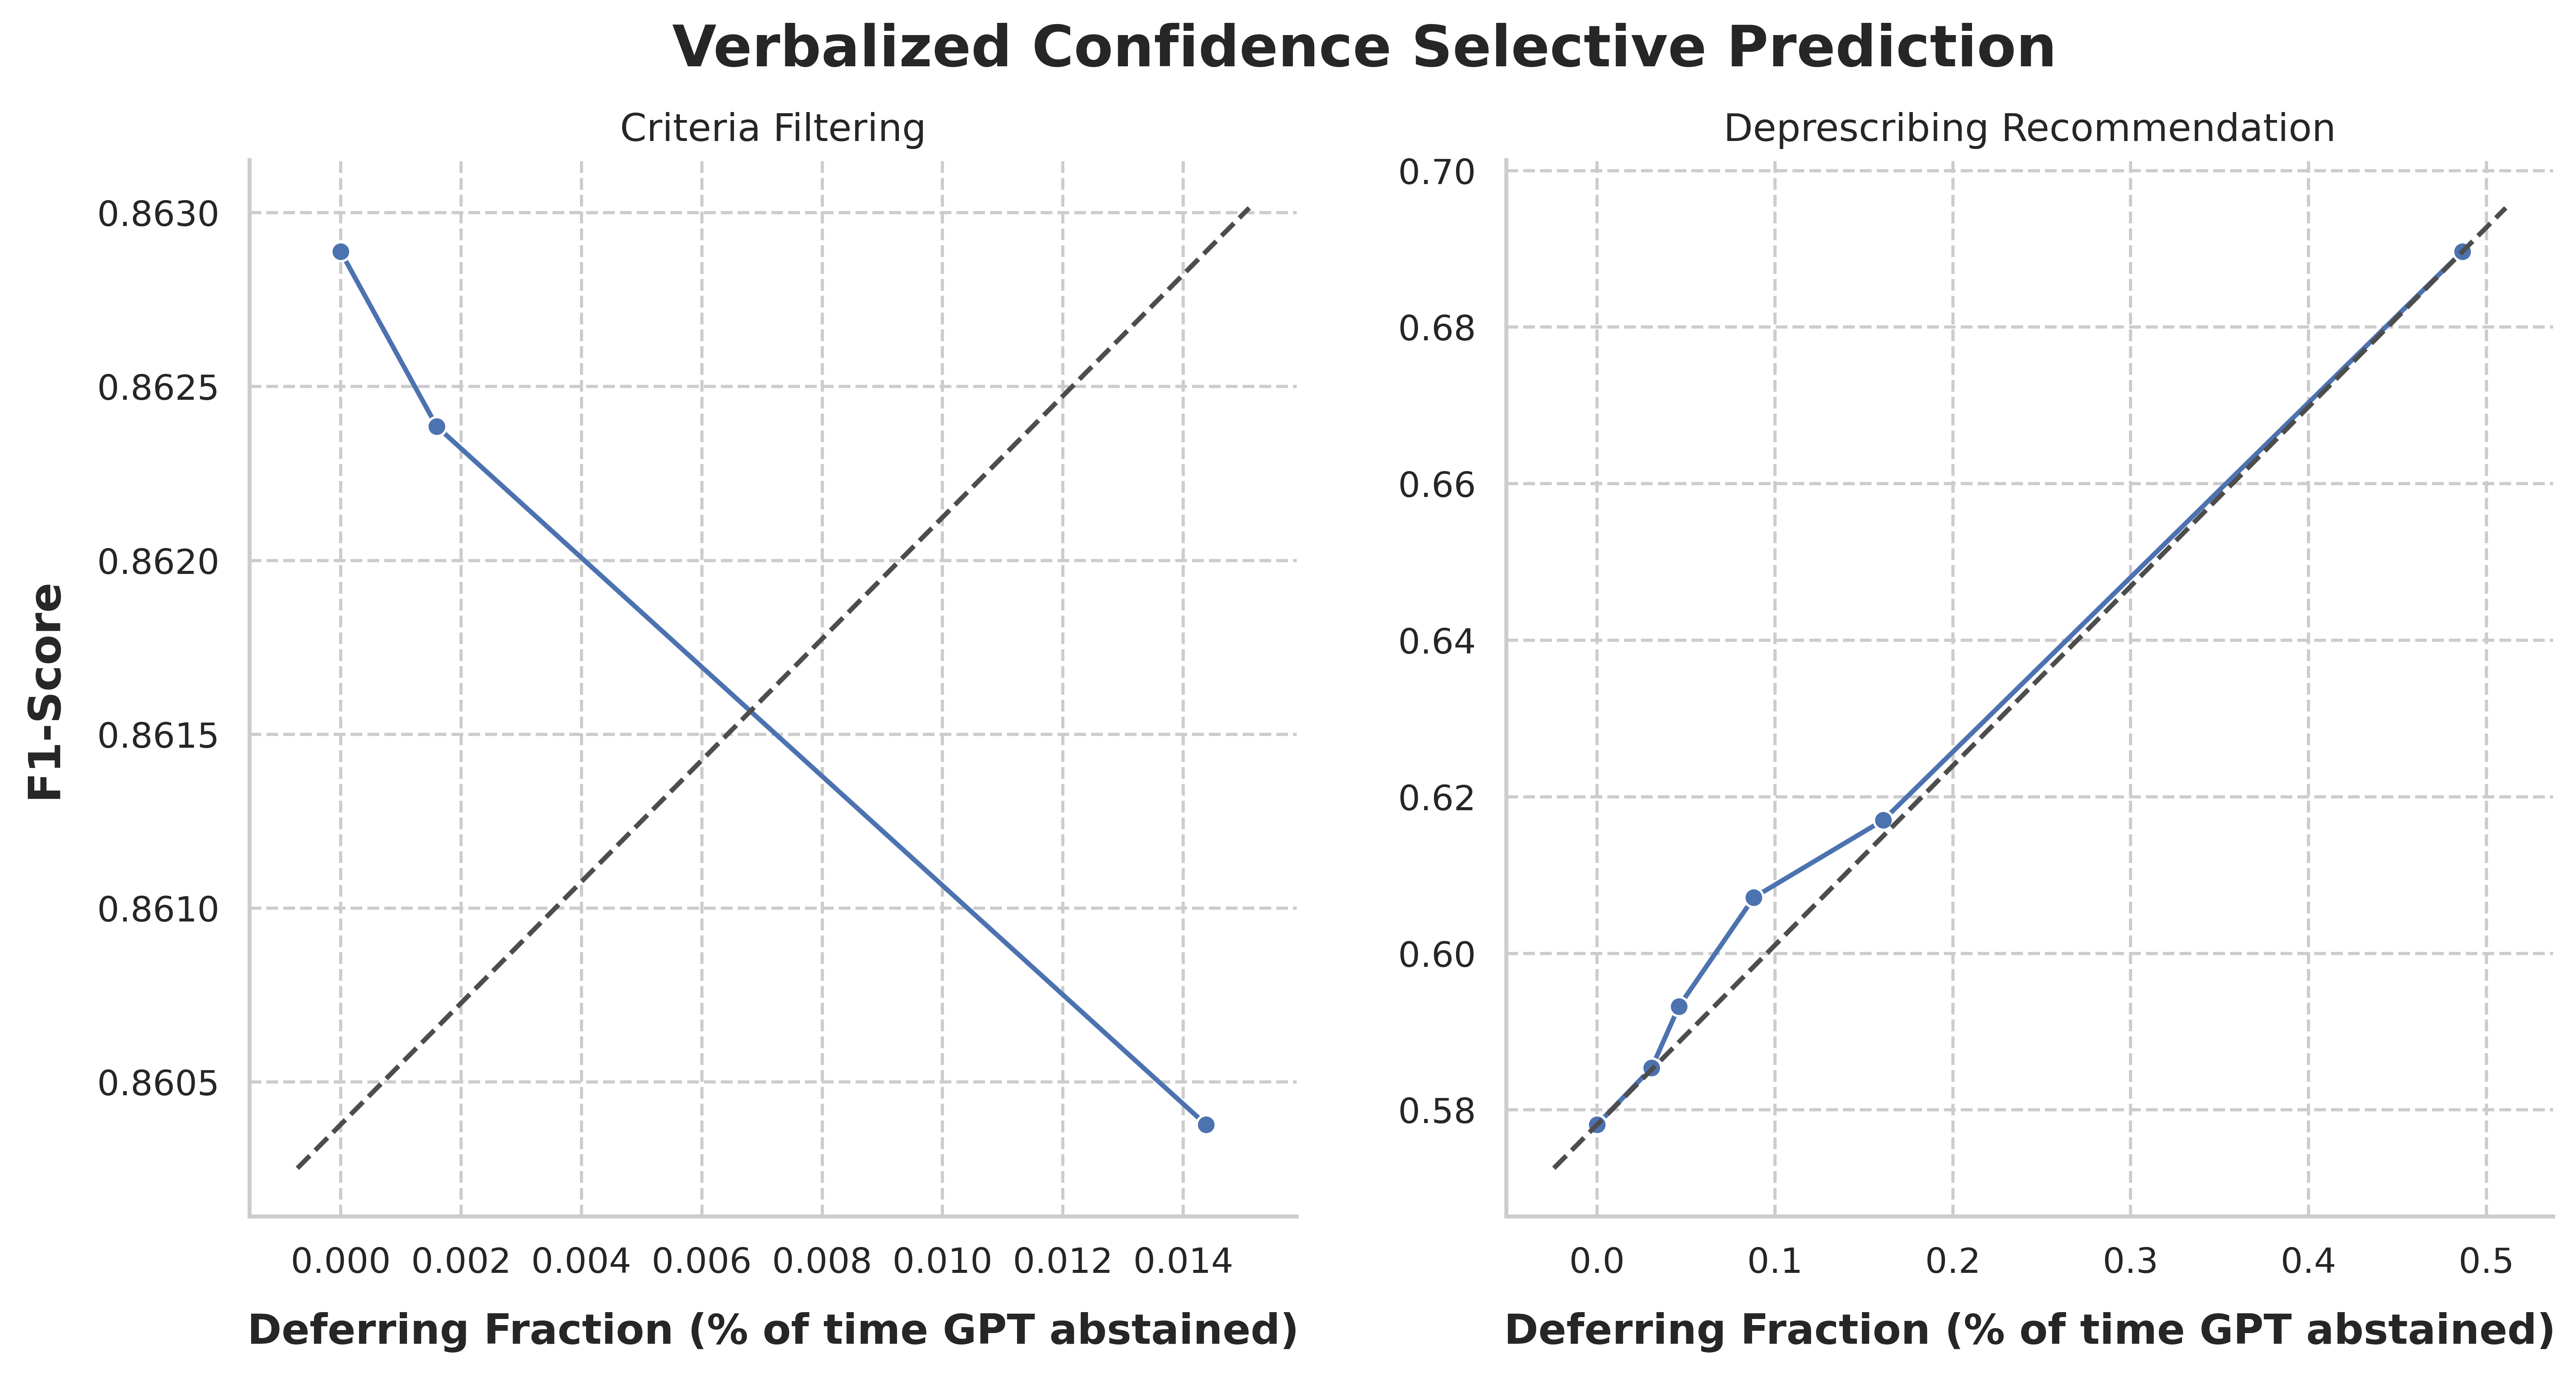
\includegraphics[width=\textwidth] {figures/aim1/selective_pred_verbconf.png}
	\caption{Range of F1-scores resulting from the application of verbalized confidence-based selective prediction for both steps of the deprescribing pipeline. The dotted line shows ideal performance as a function of deferring fraction.} \label{fig:aim1-verbconf}
\end{figure}

\section{Aim 3: Supplementary Figures}

\begin{figure}[ht!]
	\centering
	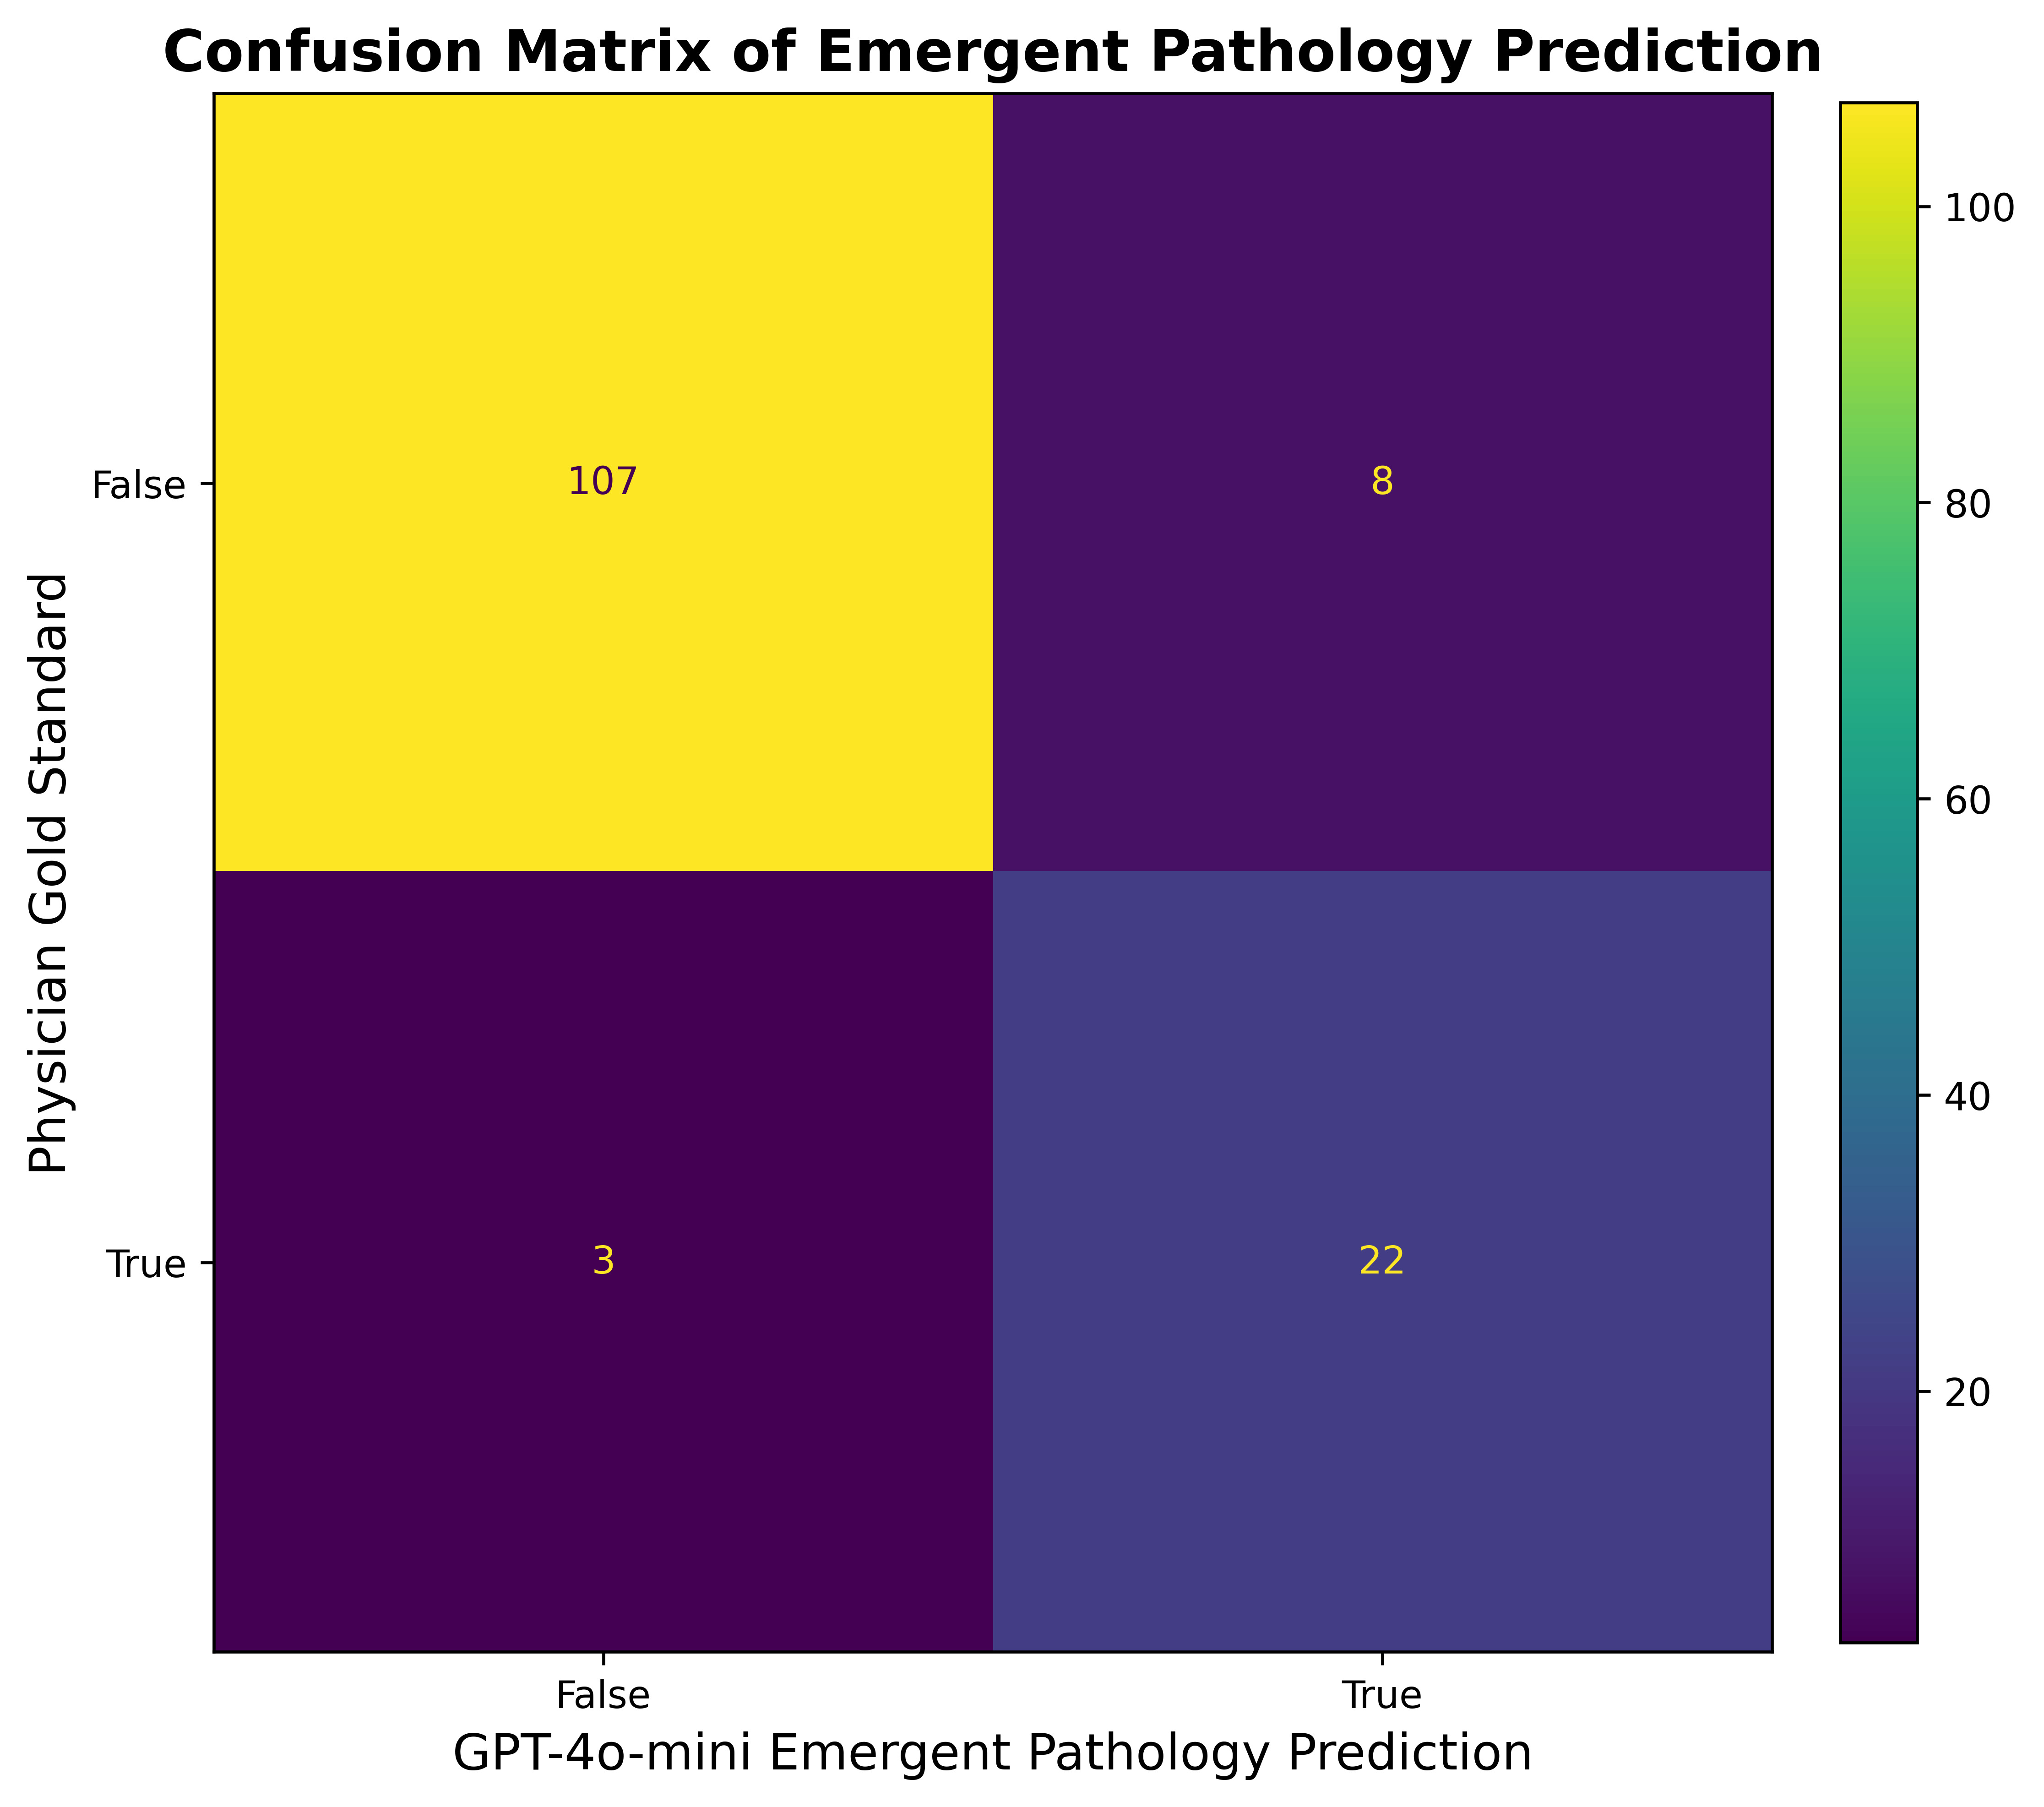
\includegraphics[width=0.85\textwidth] {figures/aim3/imaging_emergent_path_confmat.png}
	\caption{Confusion matrix comparing GPT-4o-mini's prediction of emergent pathology findings in radiology consults, compared with gold-standard physician annotations.} \label{fig:aim3-imaging-path-confmat}
\end{figure}


